
\section{Danh sách thiết bị tối thiểu, sơ đồ IP và sơ đồ đi dây}
\subsection{Danh sách các thiết bị tối thiểu}
Theo yêu cầu của dự án thực tế, Bệnh viện cần hạ tầng mạng GigaEthernet 1GbE / 10GbE/ 40GbE. Tuy nhiên, do giới hạn về thư viện thiết bị phần cứng của phần mềm mô phỏng Cisco Packet Tracer, nhóm chúng em quyết định sử dụng các thiết bị có sẵn trong thư viện giả lập (như Router 1941, Switch 3650, Switch 2960) để thiết lập mô hình. Mục đích chính là chứng minh tính đúng đắn của logic mạng, định tuyến, phân chia VLAN và các chính sách bảo mật ACL. Khi triển khai thực tế, các thiết bị này sẽ được thay thế bằng các dòng Enterprise hiện đại tương đương.
\subsubsection{Router}
Router Cisco ISR 2911: Đóng vai trò là Router biên (Edge Router) tại Trụ sở chính và các chi nhánh, chịu trách nhiệm kết nối mạng nội bộ của bệnh viện ra Internet và hệ thống mạng WAN.\\
\indent Thực hiện định tuyến động (OSPF) trên toàn mạng, thiết lập cân bằng tải (Load Balancing), cấu hình NAT, và thiết lập các kênh truyền ảo (VPN Site-to-Site bằng IPsec) để bảo mật dữ liệu y tế giữa các cơ sở.

\begin{tcolorbox}[
        enhanced,
        colback=white,
        colframe=darkgray,
        coltitle=black,
        fonttitle=\large\bfseries,
        title=Thông số kỹ thuật Router Cisco ISR 2911,
        attach boxed title to top left={xshift=5mm, yshift=-3mm},
        boxed title style={colback=white, colframe=darkgray},
        drop fuzzy shadow,
        top=4mm, bottom=2mm, left=2mm, right=2mm
    ]
        \begin{itemize}
            \item \textbf{Cổng kết nối mạng (Tích hợp):} 3 cổng Gigabit Ethernet (10/100/1000 Mbps).
            \item \textbf{Khe cắm mở rộng:} Hỗ trợ các khe cắm module EHWIC/HWIC (dùng để cắm thêm module cổng quang hoặc Serial kết nối Leased Line/MPLS).
            \item \textbf{Bộ nhớ DRAM:} 512 MB (mặc định) / Tối đa 2.5 GB.
            \item \textbf{Bộ nhớ Flash:} 256 MB (mặc định) / Tối đa 8 GB.
            \item \textbf{Tính năng nổi bật:} Hỗ trợ tăng tốc mã hóa phần cứng cho VPN, QoS nâng cao và tích hợp các tính năng bảo mật (Threat Control).
        \end{itemize}
    \end{tcolorbox}

\subsubsection{Access Point}
Access Point AP-PT: Được triển khai làm điểm truy cập không dây chủ đạo trong
toàn bộ mạng bệnh viện. Thiết bị này đảm bảo khả năng kết nối ổn định cho các thiết
bị di động, máy tính xách tay, máy trạm và các thiết bị IoT y tế tại các khu vực như
phòng khám, hành lang, khu chẩn đoán hình ảnh và khu hành chính.\\
\indent AP-PT hoạt động trên băng tần 2.4GHz, cung cấp vùng phủ sóng rộng, đảm bảo
khả năng roaming liền mạch giữa các khu vực. Tín hiệu từ các thiết bị đầu cuối được
truyền đến switch truy cập, từ đó kết nối đến hệ thống mạng lõi. Việc triển khai mạng
Wi-Fi này giúp nhân viên y tế truy cập nhanh chóng vào hồ sơ bệnh án điện tử (EHR)
và hỗ trợ truyền tải dữ liệu theo thời gian thực.
\begin{tcolorbox}[
    enhanced,
    colback=white,
    colframe=darkgray,
    coltitle=black,
    fonttitle=\large\bfseries,
    title=Thông số kỹ thuật Access Point AP-PT,
    attach boxed title to top left={xshift=5mm, yshift=-3mm},
    boxed title style={colback=white, colframe=darkgray},
    drop fuzzy shadow,
    top=4mm, bottom=2mm, left=2mm, right=2mm
]
    \begin{itemize}
        \item \textbf{Cổng kết nối:} Fast Ethernet
        \item \textbf{Băng tần hoạt động:} 2.4GHz
        \item \textbf{Chuẩn Wi-Fi hỗ trợ:} IEEE 802.11 b/g/n
    \end{itemize}
\end{tcolorbox}

\subsubsection{Firewall}
Cisco ASA 5506-X : Được sử dụng làm Firewall tại Trụ sở chính để bảo vệ mạng nội bộ khỏi các mối đe dọa từ Internet.\\
\indent Hỗ trợ tạo nhiều vùng bảo mật khác nhau như Internal, DMZ, External giúp kiểm soát chặt chẽ luồng dữ liệu ra vào. Tích hợp các tính năng tường lửa thế hệ mới (NGFW) và hỗ trợ VPN bảo mật.

\begin{tcolorbox}[
        enhanced,
        colback=white,
        colframe=darkgray,
        coltitle=black,
        fonttitle=\large\bfseries,
        title=Thông số kỹ thuật Cisco ASA 5506-X,
        attach boxed title to top left={xshift=5mm, yshift=-3mm},
        boxed title style={colback=white, colframe=darkgray},
        drop fuzzy shadow,
        top=4mm, bottom=2mm, left=2mm, right=2mm
    ]
        \begin{itemize}
            \item \textbf{Số cổng kết nối:} 8 cổng Gigabit Ethernet[cite: 3].
            \item \textbf{VLAN hỗ trợ:} Tối đa 3 VLAN[cite: 3].
            \item \textbf{Hỗ trợ VPN:} SSL VPN và IPsec VPN[cite: 3].
            \item \textbf{Giao diện quản lý:} ASDM đồ họa[cite: 3].
            \item \textbf{Tính năng bảo mật:} Lọc gói tin, bảo vệ chống DDoS, kiểm soát truy cập ứng dụng[cite: 3].
        \end{itemize}
    \end{tcolorbox}

\subsubsection{Access Switch}
Switch Cisco Catalyst 2960: Được sử dụng làm Switch truy cập (Access Switch) đặt tại các tầng (ví dụ: thiết bị \texttt{Acc-A-F1} tại Tầng 1 - Tòa A).\\
\indent Thiết bị này giúp truyền tải dữ liệu nhanh chóng giữa các khu vực chức năng như
tiếp nhận bệnh nhân, phòng chẩn đoán, khu xét nghiệm và hành chính, đảm bảo hiệu
suất và độ tin cậy cao.

\begin{tcolorbox}[
    enhanced,
    colback=white,
    colframe=darkgray,
    coltitle=black,
    fonttitle=\large\bfseries,
    title=Thông số kỹ thuật Cisco WS-C2960-24TT-L,
    attach boxed title to top left={xshift=5mm, yshift=-3mm},
    boxed title style={colback=white, colframe=darkgray},
    drop fuzzy shadow, % Hiệu ứng đổ bóng mờ
    top=4mm, bottom=2mm, left=2mm, right=2mm
]
    \begin{itemize}
        \item \textbf{Cổng Ethernet:} 24 cổng 10/100 Mbps
        \item \textbf{Cổng uplink Gigabit:} 2 cổng 10/100/1000 Mbps
        \item \textbf{Bộ nhớ DRAM:} 64 MB
        \item \textbf{Bộ nhớ Flash:} 32 MB
    \end{itemize}
\end{tcolorbox}

\subsubsection{Distribution Switch}
Distribution Switch Cisco Catalyst 3650-24PS-L: Dùng làm Switch phân phối, kết nối các Access Switch từ các tầng và khu vực để truyền dữ liệu lên mạng lõi (Core).\\
\indent Thực hiện định tuyến nội bộ giữa các VLAN (Inter-VLAN Routing), quản lý VTP, cung cấp nguồn PoE+ cho các thiết bị tầng dưới, và là điểm hội tụ băng thông.

\begin{tcolorbox}[
        enhanced,
        colback=white,
        colframe=darkgray,
        coltitle=black,
        fonttitle=\large\bfseries,
        title=Thông số kỹ thuật Cisco Catalyst 3650-24PS-L,
        attach boxed title to top left={xshift=5mm, yshift=-3mm},
        boxed title style={colback=white, colframe=darkgray},
        drop fuzzy shadow,
        top=4mm, bottom=2mm, left=2mm, right=2mm
    ]
        \begin{itemize}
            \item \textbf{Cổng Ethernet:} 24 cổng 10/100/1000 Mbps (hỗ trợ PoE+)[cite: 3].
            \item \textbf{Cổng Uplink:} 4 cổng 1G SFP (dùng để cắm cáp quang)[cite: 3].
            \item \textbf{Công suất PoE khả dụng:} 390 W[cite: 3].
            \item \textbf{Dung lượng chuyển mạch:} 88 Gbps[cite: 3].
            \item \textbf{Hiệu suất chuyển tiếp:} 41,66 Mpps[cite: 3].
            \item \textbf{Bộ nhớ:} DRAM 4 GB, Flash 2 GB[cite: 3].
        \end{itemize}
    \end{tcolorbox}
\subsubsection{Server}
Server-PT:Cung cấp các dịch vụ cốt lõi cho hoạt động của Bệnh viện (như quản lý bệnh án HIS, lưu trữ hình ảnh y tế PACS, cơ sở dữ liệu) và các dịch vụ mạng (Web, DNS, DHCP
\begin{tcolorbox}[
        enhanced,
        colback=white,
        colframe=darkgray,
        coltitle=black,
        fonttitle=\large\bfseries,
        title=Thông số kỹ thuật đề xuất cho Server (Thực tế),
        attach boxed title to top left={xshift=5mm, yshift=-3mm},
        boxed title style={colback=white, colframe=darkgray},
        drop fuzzy shadow,
        top=4mm, bottom=2mm, left=2mm, right=2mm
    ]
        \begin{itemize}
            \item \textbf{Lưu ý:} Trong Packet Tracer, nhóm sử dụng \texttt{Server-PT} làm thiết bị mô phỏng chung. Khi triển khai thực tế, Bệnh viện cần trang bị các dòng máy chủ Enterprise mạnh mẽ (ví dụ: Dell PowerEdge R740 hoặc HPE ProLiant DL380 Gen10).
            \item \textbf{Thông số cấu hình dự kiến (Tham khảo):}
            \begin{itemize}
                \item CPU: 2x Intel Xeon Scalable Processors.
                \item RAM: Tối thiểu 128 GB (Có thể mở rộng lên hàng TB cho Database).
                \item Storage: Cấu hình RAID 10 với các ổ cứng SSD NVMe tốc độ cao.
                \item Card mạng (NIC): 2x hoặc 4x cổng 10GbE / 40GbE.
            \end{itemize}
        \end{itemize}
    \end{tcolorbox}

\subsubsection{End Device}
Ngoài các thiết bị trên còn có một số thiết bị khác như: máy chủ, webcam, PC, IoT, ...  

\subsection{Sơ đồ IP}
Hệ thống mạng của bệnh viện sử dụng dải IP Private lớp A (\texttt{10.0.0.0/8}) và được quy hoạch theo mô hình phân cấp (Hierarchical IP Addressing). Cấu trúc IP được thiết kế theo cú pháp \textbf{\texttt{10.[Site].[VLAN].0}}, giúp tối ưu hóa bảng định tuyến OSPF và dễ dàng quản lý các chính sách bảo mật ACL. 

Bên cạnh đó, hệ thống áp dụng kỹ thuật chia mạng con VLSM (Variable Length Subnet Mask) để đáp ứng linh hoạt số lượng thiết bị thực tế, điển hình như việc sử dụng subnet \texttt{/22} cho VLAN Medical tại Trụ sở chính nhằm cung cấp đủ IP cho hơn 600 máy trạm.

\subsubsection{Quy hoạch IP tại Trụ sở chính - Main Site (HCMC)}
Dải mạng phân bổ cho Main Site: \textbf{10.10.0.0/16}

{
    \small % Thu nhỏ chữ một chút để bảng đẹp hơn
    \renewcommand{\arraystretch}{1.3}
    \begin{longtable}{|c|>{\raggedright\arraybackslash}p{6cm}|l|l|}
        \caption{Quy hoạch địa chỉ IP và VLAN tại Trụ sở chính (Main Site)}
        \label{tab:ip_main} \\
        \hline
        \textbf{VLAN} & \textbf{Chức năng (Phân vùng)} & \textbf{Địa chỉ mạng} & \textbf{Subnet Mask} \\
        \hline
        \endfirsthead
        
        \endhead

        \endfoot

        \hline
        \endlastfoot

        10 & Vùng phi quân sự (DMZ) & 10.10.10.0/24 & 255.255.255.0 \\
        \hline
        20 & Server Farm & 10.10.20.0/24 & 255.255.255.0 \\
        \hline
        30 & Management (Quản trị IT) & 10.10.30.0/24 & 255.255.255.0 \\
        \hline
        40 & Medical (Khu vực Y tế - 600+ hosts) & 10.10.40.0/22 & 255.255.252.0 \\
        \hline
        50 & Admin (Hành chính) & 10.10.50.0/24 & 255.255.255.0 \\
        \hline
        60 & Finance (Tài chính - Kế toán) & 10.10.60.0/24 & 255.255.255.0 \\
        \hline
        70 & IT-Ops (Vận hành IT) & 10.10.70.0/24 & 255.255.255.0 \\
        \hline
        80 & HR (Nhân sự) & 10.10.80.0/24 & 255.255.255.0 \\
        \hline
        90 & Camera (Hệ thống giám sát CCTV) & 10.10.90.0/24 & 255.255.255.0 \\
        \hline
        100 & VoIP (Hệ thống điện thoại IP) & 10.10.100.0/24 & 255.255.255.0 \\
        \hline
        110 & Guest Wi-Fi (Mạng Khách) & 10.10.110.0/23 & 255.255.254.0 \\
    \end{longtable}
}
\subsubsection{Quy hoạch IP tại các Chi nhánh phụ (Auxiliary Sites)}
Dải mạng phân bổ cho Chi nhánh DBP: \textbf{10.20.0.0/16} \\
Dải mạng phân bổ cho Chi nhánh BHTQ: \textbf{10.30.0.0/16} \\
\textit{(Do hai chi nhánh có cấu trúc tương đương nhau, quy hoạch VLAN được đồng bộ hóa để thuận tiện cho việc quản lý tập trung).}

{
    \small
    \renewcommand{\arraystretch}{1.3}
    \begin{longtable}{|c|>{\raggedright\arraybackslash}p{6cm}|l|l|}
        \caption{Quy hoạch địa chỉ IP tại các Chi nhánh (Quy ước: X=20 cho DBP, X=30 cho BHTQ)}
        \label{tab:ip_aux} \\
        \hline
        \textbf{VLAN} & \textbf{Chức năng (Phân vùng)} & \textbf{Địa chỉ mạng} & \textbf{Subnet Mask} \\
        \hline
        \endfirsthead
        
        \endhead

        \endfoot

        \hline
        \endlastfoot

        30 & Management & 10.X.30.0/24 & 255.255.255.0 \\
        \hline
        40 & Medical (Khu vực Y tế) & 10.X.40.0/23 & 255.255.254.0 \\
        \hline
        50 & Admin (Hành chính) & 10.X.50.0/24 & 255.255.255.0 \\
        \hline
        60 & Finance (Tài chính - Kế toán) & 10.X.60.0/24 & 255.255.255.0 \\
        \hline
        70 & IT-Ops (Vận hành IT) & 10.X.70.0/24 & 255.255.255.0 \\
        \hline
        80 & HR (Nhân sự) & 10.X.80.0/24 & 255.255.255.0 \\
        \hline
        90 & Camera (Hệ thống giám sát CCTV) & 10.X.90.0/24 & 255.255.255.0 \\
        \hline
        100 & VoIP (Hệ thống điện thoại IP) & 10.X.100.0/24 & 255.255.255.0 \\
        \hline
        110 & Guest Wi-Fi (Mạng Khách) & 10.X.110.0/24 & 255.255.255.0 \\
    \end{longtable}
}

% Thêm lệnh này để ngắt sang trang mới cho sạch sẽ, không bị dính chùm với phần trên


\subsection{Quy hoạch đi dây (Wiring Plan)}

Để đảm bảo hiệu năng, tính dự phòng và khả năng mở rộng cho hệ thống mạng bệnh viện, nhóm áp dụng quy hoạch đấu nối cáp theo cấu trúc phân cấp. Thay vì biểu diễn bằng hình ảnh mạng tổng thể (được trình bày chi tiết ở Bước 4), phần này quy định các chuẩn cáp và tốc độ kết nối vật lý giữa các phân lớp thiết bị trong toàn bộ hệ thống.

% Sử dụng longtable để bảng tự động chia trang mà vẫn đúng thứ tự
{
    \small
    \renewcommand{\arraystretch}{1.4}
    \begin{longtable}{|p{4.5cm}|p{3.5cm}|c|>{\raggedright\arraybackslash}p{6cm}|}
        \caption{Bảng quy chuẩn đấu nối cáp (Wiring Standards) cho hệ thống mạng}
        \label{tab:wiring_plan} \\
        \hline
        \textbf{Kết nối (Từ $\leftrightarrow$ Đến)} & \textbf{Loại cáp} & \textbf{Cổng} & \textbf{Băng thông / Ghi chú} \\
        \hline
        \endfirsthead
        
        \endhead

        \endfoot

        \hline
        \endlastfoot

        Router $\leftrightarrow$ Firewall ASA & Cáp đồng (UTP Cat6) & RJ45 & 1 Gbps (Định tuyến luồng dữ liệu bảo mật) \\
        \hline
        Firewall $\leftrightarrow$ Cụm Server (DMZ) & Cáp quang / Cat6a & SFP/RJ45 & 1 Gbps (Đảm bảo tốc độ truy xuất máy chủ) \\
        \hline
        Core/Dist Switch $\leftrightarrow$ Phân hệ Routing & Cáp quang (Fiber) & SFP & 1 Gbps (Liên kết Uplink tốc độ cao) \\
        \hline
        Distribution $\leftrightarrow$ Access Switch & Cáp quang (Fiber) & SFP & 1 Gbps (Đường Trunking truyền tải đa VLAN) \\
        \hline
        Access Switch $\leftrightarrow$ PC / Laptop & Cáp đồng (UTP Cat6) & RJ45 & 100/1000 Mbps (Kết nối thiết bị đầu cuối) \\
        \hline
        Access Switch $\leftrightarrow$ Access Point & Cáp đồng (UTP Cat6) & RJ45 & 1000 Mbps (Hỗ trợ PoE cấp nguồn cho AP) \\
        \hline
        Access Switch $\leftrightarrow$ Webcam/IoT & Cáp đồng (UTP Cat5e) & RJ45 & 100 Mbps (Cấp nguồn PoE cho thiết bị giám sát) \\
    \end{longtable}
}

\subsubsection{Kiến trúc tổng thể toàn hệ thống (High-level Topology)}

Sơ đồ tổng thể thể hiện cách hệ thống mạng của bệnh viện tương tác với môi trường Internet bên ngoài và sự phân bổ các khu vực trọng yếu. Toàn bộ lưu lượng ra/vào mạng nội bộ đều được kiểm soát bởi cụm Gateway Router và Tường lửa (Firewall ASA).

\begin{figure}[H]
    \centering
    % Nhớ đổi tên file ảnh cho đúng với file của mày
    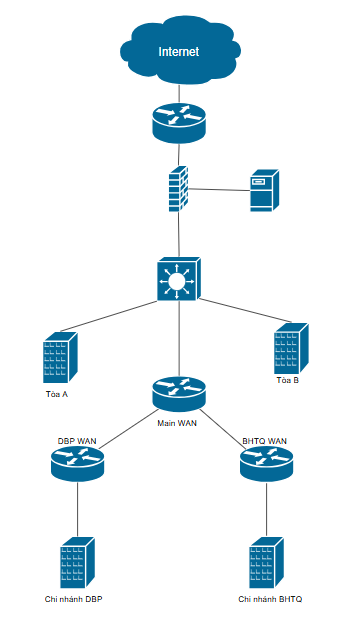
\includegraphics[width=0.5\textwidth]{Images/fullwireplan.png}
    \caption{Sơ đồ kiến trúc mạng logic tổng thể toàn hệ thống}
    \label{fig:logical_tongthe}
\end{figure}

\subsubsection{Sơ đồ chi tiết cụm Trụ sở chính (Main Site)}

Tại Trụ sở chính (HCMC), mạng được thiết kế theo mô hình Core - Distribution - Access. Switch Core (Multilayer Switch 3650) đóng vai trò trung tâm điều phối toàn bộ lưu lượng. Đặc biệt, khu vực Data Center được tách biệt hoàn toàn: vùng DMZ (đặt Web/DNS Server) cắm trực tiếp vào Tường lửa để phục vụ truy cập ngoài, trong khi Server Farm (chứa máy chủ HIS, Database nội bộ) được bảo vệ phía sau Switch Core.

\begin{figure}[H]
    \centering
    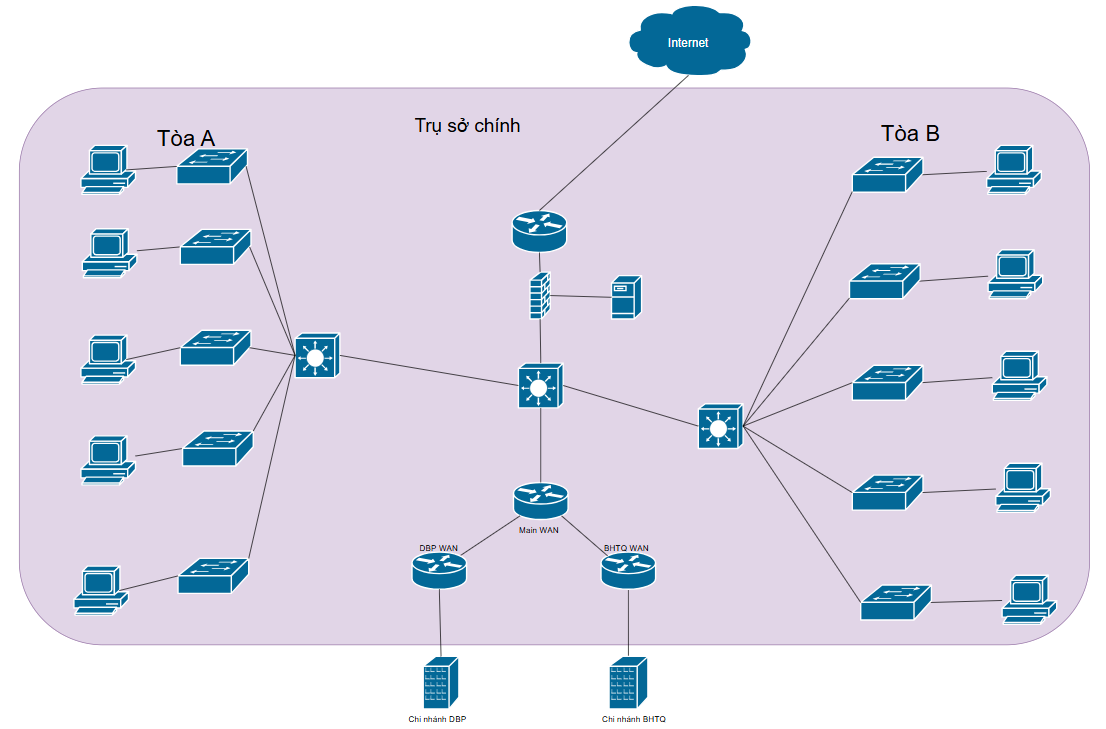
\includegraphics[width=0.95\textwidth]{Images/Maincenter.png}
    \caption{Sơ đồ chi tiết phân vùng hạ tầng mạng tại Trụ sở chính}
    \label{fig:logical_mainsite}
\end{figure}

\subsubsection{Sơ đồ chi tiết kết nối các Chi nhánh (Auxiliary Sites)}

Để đảm bảo kết nối liên tục từ Trụ sở chính đến hai chi nhánh DBP và BHTQ, nhóm sử dụng hạ tầng kết nối WAN (Wide Area Network). Các Router biên (WAN Edge Router) tại Trụ sở chính thiết lập kênh truyền tốc độ cao đến các Router đầu cuối đặt tại mỗi chi nhánh, từ đó phân phối tín hiệu xuống các Core-Switch chi nhánh.

\begin{figure}[H]
    \centering
    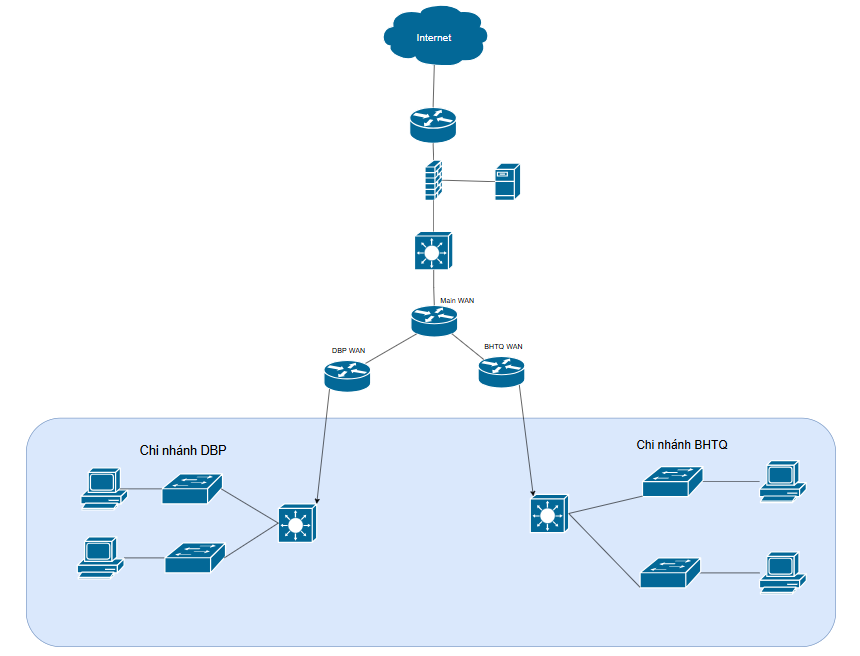
\includegraphics[width=0.95\textwidth]{Images/Chinhanh.png}
    \caption{Sơ đồ chi tiết hạ tầng mạng LAN và kết nối WAN tại các Chi nhánh phụ}
    \label{fig:logical_chinhanh}
\end{figure}